\documentclass{standalone}
\usepackage{tikz}
\usepackage{xcolor}
\usetikzlibrary{patterns, positioning}
\usetikzlibrary{shapes.misc}
\usepackage[outline]{contour}
\contourlength{1.5pt} 


\begin{document}
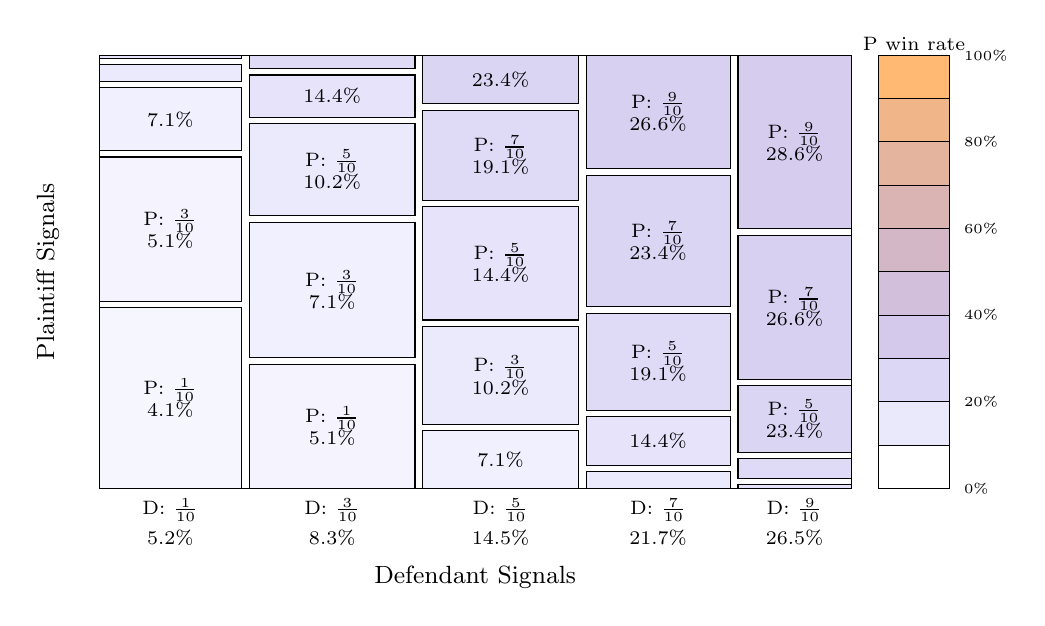
\begin{tikzpicture}
\newcommand{\DFractionOffset}{0.4}
\newcommand{\AxisLabelYAdjust}{-0.235}
\draw[draw=black] (0.6,2) rectangle (10.15,7.5);
\draw[fill=blue!96!orange!4!white!87!white, draw=black] (0.6,2) rectangle (2.4087,4.2941);
\draw (1.5043488544989276, 3.1470617565806127) node[font=\scriptsize, text=black, align=center] {P: $\frac{1}{10}$\\ 4.1\%};
\draw[fill=blue!95!orange!5!white!86!white, draw=black] (0.6,4.3741) rectangle (2.4087,6.2091);
\draw (1.5043488544989276, 5.2916270180920115) node[font=\scriptsize, text=black, align=center] {P: $\frac{3}{10}$\\ 5.1\%};
\draw[fill=blue!93!orange!7!white!86!white, draw=black] (0.6,6.2891) rectangle (2.4087,7.086);
\draw (1.5043488544989276, 6.687545822764755) node[font=\scriptsize, text=black, align=center] {7.1\%};
\draw[fill=blue!90!orange!10!white!85!white, draw=black] (0.6,7.166) rectangle (2.4087,7.381);
\draw[fill=blue!86!orange!14!white!83!white, draw=black] (0.6,7.461) rectangle (2.4087,7.5);
\draw (1.5043488544989276, 1.6) node[anchor=north, font=\scriptsize, text=black] {5.2\%};
\draw (1.5043488544989276, {1.6 + \DFractionOffset}) node[anchor=north, font=\scriptsize, text=black] {D: $\frac{1}{10}$};
\draw[fill=blue!95!orange!5!white!86!white, draw=black] (2.5087,2) rectangle (4.6115,3.5784);
\draw (3.5600995914595686, 2.7891780084511333) node[font=\scriptsize, text=black, align=center] {P: $\frac{1}{10}$\\ 5.1\%};
\draw[fill=blue!93!orange!7!white!86!white, draw=black] (2.5087,3.6584) rectangle (4.6115,5.3816);
\draw (3.5600995914595686, 4.519997303756799) node[font=\scriptsize, text=black, align=center] {P: $\frac{3}{10}$\\ 7.1\%};
\draw[fill=blue!90!orange!10!white!85!white, draw=black] (2.5087,5.4616) rectangle (4.6115,6.6332);
\draw (3.5600995914595686, 6.047406454867542) node[font=\scriptsize, text=black, align=center] {P: $\frac{5}{10}$\\ 10.2\%};
\draw[fill=blue!86!orange!14!white!83!white, draw=black] (2.5087,6.7132) rectangle (4.6115,7.2506);
\draw (3.5600995914595686, 6.981883441049107) node[font=\scriptsize, text=black, align=center] {14.4\%};
\draw[fill=blue!81!orange!19!white!82!white, draw=black] (2.5087,7.3306) rectangle (4.6115,7.5);
\draw (3.5600995914595686, 1.6) node[anchor=north, font=\scriptsize, text=black] {8.3\%};
\draw (3.5600995914595686, {1.6 + \DFractionOffset}) node[anchor=north, font=\scriptsize, text=black] {D: $\frac{3}{10}$};
\draw[fill=blue!93!orange!7!white!86!white, draw=black] (4.7115,2) rectangle (6.6846,2.7304);
\draw (5.6980708136316345, 2.3652114508669704) node[font=\scriptsize, text=black, align=center] {7.1\%};
\draw[fill=blue!90!orange!10!white!85!white, draw=black] (4.7115,2.8104) rectangle (6.6846,4.0589);
\draw (5.6980708136316345, 3.4346845834778423) node[font=\scriptsize, text=black, align=center] {P: $\frac{3}{10}$\\ 10.2\%};
\draw[fill=blue!86!orange!14!white!83!white, draw=black] (4.7115,4.1389) rectangle (6.6846,5.5793);
\draw (5.6980708136316345, 4.859141926580255) node[font=\scriptsize, text=black, align=center] {P: $\frac{5}{10}$\\ 14.4\%};
\draw[fill=blue!81!orange!19!white!82!white, draw=black] (4.7115,5.6593) rectangle (6.6846,6.803);
\draw (5.6980708136316345, 6.231159969398699) node[font=\scriptsize, text=black, align=center] {P: $\frac{7}{10}$\\ 19.1\%};
\draw[fill=blue!77!orange!23!white!80!white, draw=black] (4.7115,6.883) rectangle (6.6846,7.5);
\draw (5.6980708136316345, 7.191491175429316) node[font=\scriptsize, text=black, align=center] {23.4\%};
\draw (5.6980708136316345, 1.6) node[anchor=north, font=\scriptsize, text=black] {14.5\%};
\draw (5.6980708136316345, {1.6 + \DFractionOffset}) node[anchor=north, font=\scriptsize, text=black] {D: $\frac{5}{10}$};
\draw[fill=blue!90!orange!10!white!85!white, draw=black] (6.7846,2) rectangle (8.6129,2.2127);
\draw[fill=blue!86!orange!14!white!83!white, draw=black] (6.7846,2.2927) rectangle (8.6129,2.9108);
\draw (7.6987904765443975, 2.6017490833973946) node[font=\scriptsize, text=black, align=center] {14.4\%};
\draw[fill=blue!81!orange!19!white!82!white, draw=black] (6.7846,2.9908) rectangle (8.6129,4.225);
\draw (7.6987904765443975, 3.607924663546495) node[font=\scriptsize, text=black, align=center] {P: $\frac{5}{10}$\\ 19.1\%};
\draw[fill=blue!77!orange!23!white!80!white, draw=black] (6.7846,4.305) rectangle (8.6129,5.9793);
\draw (7.6987904765443975, 5.142187748223145) node[font=\scriptsize, text=black, align=center] {P: $\frac{7}{10}$\\ 23.4\%};
\draw[fill=blue!73!orange!27!white!79!white, draw=black] (6.7846,6.0593) rectangle (8.6129,7.5);
\draw (7.6987904765443975, 6.779664332463049) node[font=\scriptsize, text=black, align=center] {P: $\frac{9}{10}$\\ 26.6\%};
\draw (7.6987904765443975, 1.6) node[anchor=north, font=\scriptsize, text=black] {21.7\%};
\draw (7.6987904765443975, {1.6 + \DFractionOffset}) node[anchor=north, font=\scriptsize, text=black] {D: $\frac{7}{10}$};
\draw[fill=blue!86!orange!14!white!83!white, draw=black] (8.7129,2) rectangle (10.15,2.0491);
\draw[fill=blue!81!orange!19!white!82!white, draw=black] (8.7129,2.1291) rectangle (10.15,2.377);
\draw[fill=blue!77!orange!23!white!80!white, draw=black] (8.7129,2.457) rectangle (10.15,3.3042);
\draw (9.431470399873405, 2.880616933136595) node[font=\scriptsize, text=black, align=center] {P: $\frac{5}{10}$\\ 23.4\%};
\draw[fill=blue!73!orange!27!white!79!white, draw=black] (8.7129,3.3842) rectangle (10.15,5.2171);
\draw (9.431470399873405, 4.300659751797092) node[font=\scriptsize, text=black, align=center] {P: $\frac{7}{10}$\\ 26.6\%};
\draw[fill=blue!71!orange!29!white!79!white, draw=black] (8.7129,5.2971) rectangle (10.15,7.5);
\draw (9.431470399873405, 6.398553923437511) node[font=\scriptsize, text=black, align=center] {P: $\frac{9}{10}$\\ 28.6\%};
\draw (9.431470399873405, 1.6) node[anchor=north, font=\scriptsize, text=black] {26.5\%};
\draw (9.431470399873405, {1.6 + \DFractionOffset}) node[anchor=north, font=\scriptsize, text=black] {D: $\frac{9}{10}$};
\node[font=\small, text=black] at (5.375, {1.1 + \AxisLabelYAdjust}) {Defendant Signals};
\node[font=\small, text=black, rotate=90] at (-0.050000000000000044, 4.75) {Plaintiff Signals};
\draw[draw=black] (10.5,2) rectangle (11.4,7.5);
\draw (10.95, 7.65) node[font=\scriptsize, text=black] {P win rate};
\draw[fill=blue!100!orange!0!white!88!white, draw=black] (10.5,2) rectangle (11.4,2.55);
\draw[fill=blue!89!orange!11!white!84!white, draw=black] (10.5,2.55) rectangle (11.4,3.1);
\draw[fill=blue!78!orange!22!white!81!white, draw=black] (10.5,3.1) rectangle (11.4,3.65);
\draw[fill=blue!67!orange!33!white!77!white, draw=black] (10.5,3.65) rectangle (11.4,4.2);
\draw[fill=blue!56!orange!44!white!73!white, draw=black] (10.5,4.2) rectangle (11.4,4.75);
\draw[fill=blue!44!orange!56!white!70!white, draw=black] (10.5,4.75) rectangle (11.4,5.3);
\draw[fill=blue!33!orange!67!white!66!white, draw=black] (10.5,5.3) rectangle (11.4,5.85);
\draw[fill=blue!22!orange!78!white!62!white, draw=black] (10.5,5.85) rectangle (11.4,6.4);
\draw[fill=blue!11!orange!89!white!59!white, draw=black] (10.5,6.4) rectangle (11.4,6.95);
\draw[fill=blue!0!orange!100!white!55!white, draw=black] (10.5,6.95) rectangle (11.4,7.5);
\draw (11.46, 2) node[anchor=west, font=\tiny, text=black] {0\%};
\draw (11.46, 3.1) node[anchor=west, font=\tiny, text=black] {20\%};
\draw (11.46, 4.2) node[anchor=west, font=\tiny, text=black] {40\%};
\draw (11.46, 5.3) node[anchor=west, font=\tiny, text=black] {60\%};
\draw (11.46, 6.4) node[anchor=west, font=\tiny, text=black] {80\%};
\draw (11.46, 7.5) node[anchor=west, font=\tiny, text=black] {100\%};


\end{tikzpicture}
\end{document}